% =====================================================================
% Clase -- Geometría 5° -- Trimestre I -- Semana 05
% Sesión 004 (lun 28 sep., 06:55, 55 min)
% Tema: El plano cartesiano
% Subtema: Ejes, origen y cuadrantes
% Hilo conductor del trimestre I: «Cali, mi ciudad»
% Tema 2 de la guía: El plano cartesiano (tema:plano)
% Material del docente (no se entrega a los estudiantes).
% =====================================================================
\documentclass[11pt]{article}
\makeatletter\def\input@path{{../../../../../plantillas/estilo/}}\makeatother
\usepackage{mmcantillo}
\guiadelestudiante{../../guia-didactica/guia-periodo-I-ubicacion}

\tipodocumento{Clase}
\asignatura{Geometría}
\titulo{Semana 5: los cuatro barrios del plano}
\grado{5°}
\periodo{I}

% DBA: matematicas grado 5 · DBA 7 — Identifica, describe y representa figuras
% bidimensionales, y establece relaciones entre ellas usando sistemas de coordenadas.
% Evidencia de esta sesión: ubicar y leer puntos en el plano cartesiano completo (con
% coordenadas negativas), nombrando ejes, origen y cuadrantes, que es la base para describir
% figuras con coordenadas en las sesiones siguientes.

\begin{document}

\encabezado*

\begin{center}
{\renewcommand{\arraystretch}{1.3}
\begin{tabularx}{\linewidth}{@{}l l l X l@{}}
  \toprule
  \textbf{Sesión} & \textbf{Fecha} & \textbf{Min} & \textbf{Subtema} & \textbf{Entregables}\\
  \midrule
  004 & lun 28 sep., 06:55 & 55 & Ejes, origen y cuadrantes & Se deja tarea (5 pts)\\
  \bottomrule
\end{tabularx}}
\end{center}

Hasta ahora hemos ubicado puntos con números positivos, como en el mapa del colegio. Hoy el
plano se completa: aparecen los números negativos, los dos ejes se cruzan en un punto llamado
origen y el plano queda partido en cuatro regiones. Siguiendo el hilo \emph{Cali, mi ciudad},
el origen será la torre de la iglesia de La Ermita y los cuatro cuadrantes, los cuatro rumbos
de la ciudad. Referencia: \refguia{tema:plano}.

% ---------------------------------------------------------------------
\seccion{Sesión 004 — lunes 28 de septiembre · 06:55 · 55 min}

\textbf{Objetivo.} Nombrar los ejes y el origen, ubicar puntos con coordenadas positivas y
negativas, y decir en qué cuadrante queda un punto mirando solo sus dos signos.

\textbf{Materiales.} Cuadrícula grande en el tablero; regla; cuaderno cuadriculado; la guía.

\begin{center}
{\renewcommand{\arraystretch}{1.3}
\begin{tabularx}{\linewidth}{@{}l l X@{}}
  \toprule
  \textbf{Momento} & \textbf{Min} & \textbf{Actividad}\\
  \midrule
  Enganche & 0--8 & En el tablero, la cuadrícula solo con la esquina de arriba a la derecha.
    «Si La Ermita es el origen, ¿cómo escribimos un lugar que queda al \emph{occidente}?»
    Nadie puede: hacen falta números negativos. Se prolongan los dos ejes hacia el otro lado y
    el plano queda completo.\\
  Los nombres & 8--20 & Eje $x$ (horizontal, el de la izquierda–derecha), eje $y$ (vertical),
    origen $(0,0)$ donde se cruzan. Escribir los cuatro cuadrantes con números romanos,
    empezando arriba a la derecha y girando \emph{al contrario} de las manecillas del reloj:
    I, II, III, IV. Hacer la tabla de signos: I es $(+,+)$; II, $(-,+)$; III, $(-,-)$; IV,
    $(+,-)$.\\
  Ubicar y leer & 20--35 & Cada estudiante dibuja los ejes en su cuaderno y ubica seis puntos
    que dicta la docente, uno por cuadrante y dos sobre los ejes. Se revisa en el tablero.
    Regla de oro que se repite en voz alta: \textbf{primero se camina en horizontal y después
    en vertical}.\\
  Los que no tienen cuadrante & 35--45 & Los puntos $(0,-4)$, $(-5,0)$ y el origen no están en
    ningún cuadrante: están \emph{sobre} los ejes, que son la frontera. Compararlo con quien
    vive justo en la esquina entre dos barrios. Esta idea se les olvida siempre; por eso va en
    la tarea.\\
  Juego de cierre & 45--55 & «Adivina el cuadrante»: la docente dice dos signos —«menos, más»—
    y el salón responde el número romano; después al revés. Tres rondas rápidas. Se deja la
    tarea (5 puntos).\\
  \bottomrule
\end{tabularx}}
\end{center}

\textbf{Figura para el tablero: los cuatro cuadrantes.}

\begin{center}
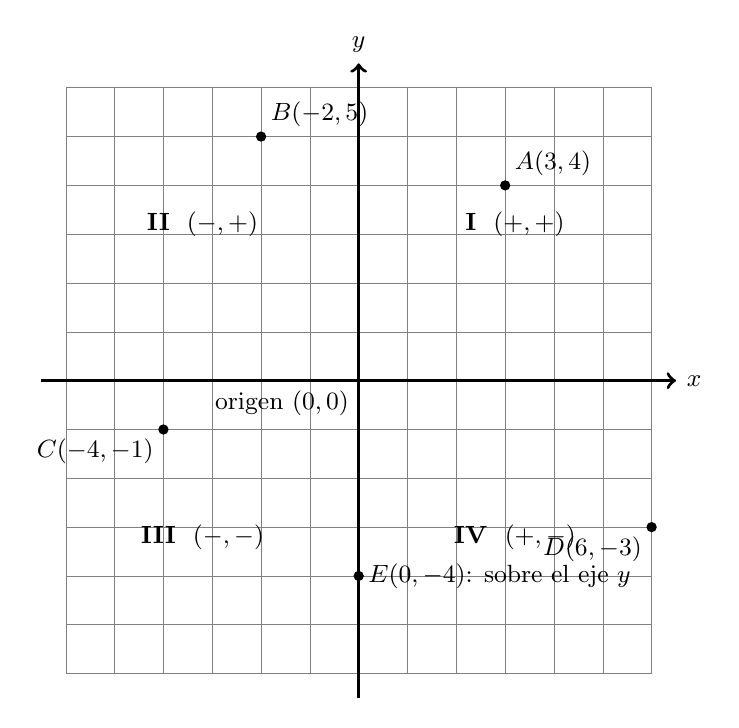
\begin{tikzpicture}[scale=0.62, every node/.style={font=\small}]
  \draw[help lines, step=1] (-6,-6) grid (6,6);
  \draw[->, very thick] (-6.5,0) -- (6.5,0) node[right] {$x$};
  \draw[->, very thick] (0,-6.5) -- (0,6.5) node[above] {$y$};
  \node[below left] at (0,0) {origen $(0,0)$};
  \node at (3.2,3.2) {\textbf{I} \ $(+,+)$};
  \node at (-3.2,3.2) {\textbf{II} \ $(-,+)$};
  \node at (-3.2,-3.2) {\textbf{III} \ $(-,-)$};
  \node at (3.2,-3.2) {\textbf{IV} \ $(+,-)$};
  \fill (3,4) circle (3pt) node[above right] {$A(3,4)$};
  \fill (-2,5) circle (3pt) node[above right] {$B(-2,5)$};
  \fill (-4,-1) circle (3pt) node[below left] {$C(-4,-1)$};
  \fill (6,-3) circle (3pt) node[below left] {$D(6,-3)$};
  \fill (0,-4) circle (3pt) node[right] {$E(0,-4)$: sobre el eje $y$};
\end{tikzpicture}
\end{center}

\begin{nota}
\textbf{Dónde suele trabarse.} En dos cosas. La primera, invertir el orden de la pareja: se
arregla repitiendo «horizontal y después vertical» cada vez, sin excepción. La segunda, querer
meter en un cuadrante los puntos que están sobre un eje; ahí ayuda la imagen de la frontera
entre dos barrios: se está en el límite, no adentro de ninguno.
\end{nota}

\begin{nota}
\textbf{Sobre el nombre.} Si alguien pregunta de dónde sale «cartesiano»: de René Descartes,
un pensador francés del siglo \textsc{xvii} a quien se le ocurrió describir la geometría con
números. La anécdota de que lo pensó mirando una mosca en el techo de su cuarto es bonita,
pero probablemente no es cierta; se puede contar diciendo justamente eso.
\end{nota}

\end{document}
